\chapter{Model platformy}
Pierwszym krokiem do stworzenia modelu dynamicznego, jest stworzenie modelu kinematycznego, aby móc porównać z nim tworzony model dynamiczny, oraz fizyczną platformę,
w celu weryfikacji poprawności działania.
Dzięki temu można łatwo oszacować, jak bardzo błędy symulacji, oraz błędy niedoskonałości fizycznego modelu odstają od matematycznych wyliczeń.

Dodatkowo, stworzenie modelu platformy kinematycznej pozwala na proste odrzucanie niedziałających implementacji modelu kinematycznego.
Model platformy kinematycznej ma także kluczowe zastosowanie w odometrii.

\begin{figure}[H]
\centering
 \includegraphics[width=0.8\textwidth]{graphics/base_dims.pdf}
\caption{Wielkości używane we wzorach.}
\label{fig:base_dims}
\end{figure} 

\begin{table}
\centering
\begin{tabular}{c c l}
Oznaczenie & Wartość & Opis \\
\hline
$r$ & 0,1 m & Promień koła w najszerszym miejscu na środku. \\
$a$ & 0,76 m & Szerokość platformy między środkami kół tej samej osi. \\
$b$ & 0,72 m & Długość platformy między środkami kół tego samego boku. \\
$\omega_i$ & & Prędkość kątowa każdego z kół. \\
$v_x$ & & Prędkość transwersalna w osi X. \\
$v_y$ & & Prędkość transwersalna w osi Y. \\
$\omega_z$ & & Prędkość kątowa w osi Z, wektor skierowany w górę. \\
\end{tabular}
\caption{Opisy i wartości symboli używanych we wzorach i rysunkach.}
\label{tab:dims}
\end{table}

\section{Sposób zapisu w formacie SDF}
\label{sec:sdf}
	\emph{Simulation Description Format} (SDF) jest formatem XML, pozwalającym na określenie elementów i zależności pomiędzy nimi w przestrzeni trójwymiarowej, 
	w szczególności budowy i rozmieszczenia robotów.
	Powstał jako zamiennik poprzedniego formatu URDF ze względu na jego skomplikowaną semantykę i brak możliwości określania środowiska wokół robotów, 
	na przykład rozmieszczenie elementów na symulowanej scenie, określania wyglądu i fizycznego zachowania się materiałów itp.

	W przeciwieństwie do poprzednika zapisującego model w przestrzeni drzewiastej, SDF równolegle określa wszystkie składowe modelu, 
	oraz zależności między nimi, jak więzy i względne pozycje.
	Model składowych robota ma strukturę gwiazdową. Jeden element, \texttt{model}, jest nadrzędny, wszystkie składowe są logicznie rozmieszczone równolegle.
	Specjalnie opisane więzy definiują interakcje pomiędzy elementami.
	Jako model, standard rozumie nie tylko roboty, ale także obiekty typu przeszkody, źródła światła, elementy animowane i tym podobne.
	Standard jest dobrze opisany na ich stronie internetowej \cite{sdf_website}.

	Element typu \texttt{world}, równoległy do modeli, zawiera informacje o środowisku symulacji.
	Dodatkowo można dodać informację o ustawieniach maszyny symulującej fizykę, wyglądzie sceny, wietrze, grawitacji, polu magnetycznym itp.

	W każdym z modeli, zawiera się nazwa, domyślna pozycja, sposób traktowania przez symulator i wtyczki programów obsługujących zaawansowane zachowanie modelu,
	opisane w równoległych do składowych elementach, ale jako że wszystkie te mogą wystąpić tylko raz, należy traktować je jako część elementu \texttt{model}.
	Model, lub jego fragment, może być zaimportowany z innego pliku, lecz nie zmieni to struktury gwiazdowej, a co za tym idzie, może dojść do utraty informacji.
	Ten przypadek zachodzi przy modelach czujników laserowych, opisanych w rozdziale \ref{sec:monokl}.

	Model zawiera w sobie równolegle wszystkie elementy typu \texttt{link}, każdy z nich jest osobną, kompletną częścią robota, na przykład kołem, 
	fragmentem ramienia chwytaka, kadłubem, czujnikiem.
	Składowa w sobie informacje o pozycji względem lokalnego środka układu współrzędnych modelu, masie, kształcie, fizycznym kształcie, materiale fizycznym i wyglądzie.
	Pozwala na dodanie elementów reprezentujących źródła dźwięku, czujniki, baterie itp.

	Same elementy zawierają jedynie informacje o swoim początkowym umiejscowieniu w modelu, ale nie o sposobie poruszania się i nałożonych więzach.
	Do tego potrzebne są, równoległe do elementów modelu, typy \texttt{joint} określające typ więzów, osie, współczynniki sprężystości, wytrzymałość, siłę silników.
	Każde połączenie określa, między jakimi obiektami się łączy.
	
	\begin{figure}[H]
	\dirtree{%
	.1 sdf.
	.2 world\DTcomment{Opis przestrzeni symulacji}.
	.2 model\DTcomment{Model w przestrzeni}.
	.3 plugin\DTcomment{Program sterujący modelem}.
	.3 link\DTcomment{Składowa modelu}.
	.4 collision\DTcomment{Fizyczny kształt składowej}.
	.4 visual\DTcomment{Siatka definiująca wygląd składowej}.
	.4 sensor\DTcomment{Czujnik w składowej}.
	.5 plugin\DTcomment{Program sterujący czujnikiem}.
	.3 joint\DTcomment{Wiąz pomiędzy składowymi}.
	}
	\caption{Najważniejsze elementy formatu SDF.}
	\label{fig:sdf_dir}
	\end{figure} 
	
\section{Model kinematyczny}
	\label{sec:pseudovelma}
	Kinematyka to nauka o ruchach obiektów na podstawie nadanych wektorów prędkości.
	Pomija ona takie aspekty jak masa, moment bezwładności, czy siły.
	
	Model kinematyczny jest sterowany funkcjami matematycznymi, 
	zamieniającymi prędkość kątową kół platformy na prędkości transwersalne geometrycznego środka platformy w układzie współrzędnych lokalnych, oraz jego prędkość kątową. 
	Symulator pozwala również na całkowanie tego ruchu, aby uzyskać aktualną pozycję platformy.
	
	Funkcje tłumaczące prędkości kół najwygodniej zapisać w postaci macierzowej, podobnie do tego, jak opisano w \cite{wheels}. 
	Wzór powtarza się w wielu innych pracach naukowych, a jego dokładny kształt zależy od kolejności numerowania kół i interpretacji wymiarów.
	Dla opisanego tutaj przypadku, (stałe zdefiniowane są w tabeli \ref{tab:dims}, numerowanie kół na rysunku \ref{fig:base_dims}):
	
	\begin{equation}
	\begin{bmatrix}
	v_x \\
	v_y \\
	\omega_z \\
	\end{bmatrix}
	=
	\frac{r}{4}
	\begin{bmatrix}
	-1 & 1 & -1 & 1 \\
	1 & 1 & 1 & 1 \\
	\frac{2}{a+b} & \frac{-2}{a+b} & \frac{-2}{a+b} & \frac{2}{a+b} \\
	\end{bmatrix}
	\begin{bmatrix}
	\omega_1 \\
	\omega_2 \\
	\omega_3 \\
	\omega_4 \\
	\end{bmatrix}
	\end{equation}
	
	Uzyskane wartości należy przemnożyć przez odpowiednie wektory jednostkowe, obrócić względem lokalnego układu współrzędnych dla modelu i zastosować w funkcjach nadających prędkości bryle.

	Ponieważ sterowanie pozycją modelu kinematycznego odbywa się wyłącznie poprzez wzory matematyczne, w jego symulacji nie uczestniczy maszyna symulacyjna fizyki.
	Taki model nie reaguje na kolizje z innymi obiektami, nie reaguje na różnicę terenu i nie używa informacji o współczynnikach tarcia materiałów, jak model dynamiczny.

	Nazwa kodowa \texttt{pseudovelma} odnosi się do tego, że jest to nieprawdziwy ruch sterowany z zewnątrz, a nie prawdziwa symulacja.

	\subsection{Problemy implementacji}
		Gazebo nie ma zaimplementowanego pełnego wsparcia dla standardu SDF.
		W szczególności nie działa struktura elementów \texttt{frame}, odpowiadająca za transformacje obiektów względem innych obiektów.
		Nie jest to zapisane w dokumentacji, a jedynie zgłoszone od kilku lat w systemie kontroli wersji jako błędy.

		Oznacza to, że wszystkie elementy typu \texttt{link}, będąc dziećmi \texttt{model}, nie zachowują swojej pozycji w lokalnym układzie współrzędnych.
		Powoduje to, że nadając prędkość kątową modelowi za pomocą funkcji, nadajemy ją każdej składowej osobno.
		Każde z kół i dwie części bazy, obracają się zgodnie z zadanymi wartościami, ale ich środki pozostają w miejscu w którym rozpoczęły symulację,
		ignorując kompletnie pozycję zdefiniowaną dla elementu rodzica \texttt{model}.
		
		Z punktu widzenia symulacji fizycznej ma to sens, gdyż nie można zakładać że składowe modelu są w jakikolwiek sposób podłączone do jego głównej części
		(która wcale nie musi mieć zdefiniowanego kształtu fizycznego), to wprowadzałoby także nieścisłości w typie połączenia, niektóre elementy powinny być przecież ruchome.

		Aby przeciwdziałać temu zjawisku, należy przenieść zawartość elementów \texttt{link} do elementu \texttt{model} i ustawić je jako \texttt{visual} elementu \texttt{model}.
		W ten sposób traktowane są jako część renderowana modelu, a nie osobne składowe.
		Nie można użyć tutaj więzów statycznych, gdyż te są wykorzystywane przez maszynę symulacyjną fizyki i ignorowane są przy kinematycznym ruchu.

		Powstała niedogodność jest taka, że ciężej jest sterować obrotem elementów \texttt{visual}, gdyż są zarządzane przez kompletnie inny system symulatora,
		służący do graficznego renderowania sceny.
		Oczywiście ma to znaczenie jedynie kosmetyczne, gdyż w żaden sposób nie wpływa na ruch modelu bazy.

	\subsection{Komunikacja}
		Komunikacja programu sterującego platformą odbywa się przez wbudowane z ROSa narzędzie \emph{topic}.

		Wiadomość zawierająca dane prędkości kół czterokołowego robota nie mieści się w standardzie, zatem został stworzony specjalny typ \texttt{omnivelma\_msgs/Vels}.
		Ta stryktura zawiera cztery wartości zmiennoprzecinkowe podwójnej precyzji, oznaczające prędkości w $\frac{rad}{s}$.

		Program w każdym cyklu symulacji nadaje wiadomości:
		\begin{itemize}
		\item \texttt{geometry\_msgs/PoseStamped} z aktualną pozycją i rotacją platformy, oraz nagłówkiem z identyfikatorem i czasem nadania pakietu.
		\item \texttt{geometry\_msgs/TwistStamped} z aktualną prędkością platformy, oraz identycznym nagłówkiem.
		\item \texttt{nav\_msgs/Odometry} z obiema powyższymi danymi i nagłówkiem. Służy przy obliczaniu ruchów platformy na podstawie enkoderów kół.
		\end{itemize}
		Ponadto program przyjmuje dane:
		\begin{itemize}
		\item \texttt{omnivelma\_msgs/Vels} z zadanymi prędkościami kół.
		\end{itemize}

	\subsection{Zachowanie}
		Platforma ignoruje kompletnie otoczenie, poruszając się przez inne obiekty na scenie.
		Po nadaniu stałych prędkości kół, następuje ruch po okręgach zgodnie z rysunkiem \ref{fig:mecanum_dirs}.

		Program sterujący, co każdą klatkę symulacji (okres zależy od zasobów procesorowych komputera), zwraca aktualną pozycję i rotację, 
		działając jak układ całkujący funkcje ruchu z powyższej macierzy.

\section{Model dynamiczny}
	\label{sec:omnivelma}
	Wykorzystując maszynę do symulacji fizyki, można umieścić w niej model określający kształty, masy i zależności pomiędzy składowymi modelu, 
	następnie nadać elementom wirtualne siły i otrzymać przybliżone wyniki do tego, jak zachowywałaby się rzeczywista platforma.

	Wszystkie programy i definicje związane z tym modelem noszą nazwę \texttt{omnivelma}, co nawiązuje do wielokierunkowości ruchów robota manipulującego, którego podstawa ma transportować.

	Robot jest bryłą, na którą składają się następujące części składowe:
	\begin{itemize}
	\item Główna część trzonu.
	\item Ruchoma, mniejsza część trzonu z przodu robota.
	\item 4 koła, 2 podłączone do głównej części, a 2 do przedniej.
	\item Po 12 rolek na każdym kole.
	\item Przegub zawiasowy, łączący dwie części podstawy.
	\item 4 przeguby zawiasowe z silnikami, łączące części bazy z kołami.
	\item 12 przegubów zawiasowych na każdym kole, łączących koła z rolkami.
	\end{itemize}

	Jest to dość skomplikowany obiekt do symulacji, dlatego należy skłonić się do znalezienia sposobu na uproszczenie modelu, w celu zmniejszenia ilości obliczeń symulatora
	i błędów reprezentacji liczb zmiennoprzecinkowych.

	Istnieje wiele podejść do stworzenia odpowiedniego modelu. Każde z nich było proponowane na różnych forach przez osoby symulujące podobne bazy, a także w zawartej bibliografii.
	
	Jednak idealne rozwiązanie nigdy nie zostało znalezione.
	Działający w tym przypadku sposób, także nie został wcześniej sprawdzony.

	\subsection{Jak największe zbliżenie do oryginału}
		Wspomniany wyżej sposób jest najbardziej wymagającym obliczeniowo, ale także najprostszym z możliwych.
		Należy stworzyć elementy składowe systemu i nadać im fizyczny kształt za pomocą odpowiedniej siatki trójkątów.
		Kształt obiektów może być także ustalony jednym prymitywów, jak sześcian, kula, łamana, walec i płaszczyzna.
		Takie przybliżenie znacznie przyspiesza obliczenia, gdyż może być specjalnie traktowane przez algorytmy.

		Słabym punktem tego rozwiązania jest fakt, że rolki są niestandardowym kształtem, opisanym dokładniej w \cite{rollers}, 
		którego dokładność jest bardzo wysoce wymagana dla zmniejszenia niedokładności ruchów.
		Przybliżenie jej walcem powoduje problemy przy przenoszeniu ciężaru na kolejną rolkę, gdyż koło będzie musiało przez chwilę oprzeć się o krawędź.
		Taki model samoczynnie drgałby przy obrocie koła, zwiększając tym samym i tak duże niedokładności. 
		Podejście to zostało także zaproponowane w innej pracy naukowej \cite{modelling_ways}.

		Przybliżenie rolki siatką, jedynie zmniejsza powyższy efekt, gdyż sama siatka zbudowana jest z prostych odcinków.
		Zwiększając jej gęstość można teoretycznie poprawić jakość symulacji, kosztem olbrzymiego skoku ilości obliczeń, każde obarczone błędami liczbowymi.
		Kalkulowanie kolizji fizycznej siatek jest najdroższe ze wszystkich obliczeń kolizji w maszynach symulacji fizyki.

	\subsection{Resetowanie pozycji koła}
		Ten sposób został użyty w modelach w symulatorze V-Rep.

		Polega on na tym, iż koło, podłączone do bazy, posiada przegub zawiasowy, obrócony pod kątem 45° w stosunku do osi koła, tak aby był równolegle do aktualnie dolnej rolki.
		Do tego przegubu podłączona jest kula reagująca z podłożem, którą to w każdej iteracji symulacji należy zresetować do pozycji wyjściowej, razem z przegubem.
		Kula jest prymitywem i obliczenia jej kolizji są najmniej wymagające obliczeniowo dla maszyny symulacyjnej.

		\begin{figure}[H]
		\dirtree{%
		.1 kadłub\DTcomment{Podstawa bazy}.
		.2 przegub z silnikiem\DTcomment{Nadaje moment obrotowy na żądanie}.
		.3 wirtualne koło\DTcomment{Obiekt bez kształtu, obraca się jak koło}.
		.4 siatka\DTcomment{Odpowiada za wygląd obiektu koła}.
		.4 przegub 45°\DTcomment{Obrócony pod kątem 45°}.
		.5 kula kształtu\DTcomment{Uczestniczy w symulacji fizyki}.
		}
		\caption{Zagnieżdżenie obiektów koła z resetowaną symulacją rolki.}
		\label{fig:vrep_wheel}
		\end{figure}

		Wywołuje to takie działanie, jak gdyby koło w danej chwili mogło obracać się w dwóch kierunkach, tak jak aktualnie najniższa rolka i tak jak wymusza to na kole 
		symulator silnika mechanicznego.
		Przez następną klatkę symulacji, model zachowuje się poprawnie, aż obrót głównej osi zaczyna negatywnie wpływać na symulację,
		zmieniając kąt wewnętrznego przegubu, przez co przestaje być równoległy do dolnej rolki.
		Zanim jednak ten efekt się nasili, jego rotacja jest przywracana do pozycji początkowej.
		Ponieważ jest to wywoływane poprzez zmianę rotacji, a nie nadanie momentu obrotowego obiektowi, 
		maszyna symulacyjna nie bierze w takim przypadku pod uwagę tarcia kuli o podłoże. 

		Niestety, nie jest możliwe uzyskanie tego rozwiązania wprost w Gazebo, gdyż struktura drzewiasta obiektów nie jest zaimplementowana, jak to wcześniej zostało opisane.
		Co więcej, metody natychmiastowo zmieniające pozycje obiektu nie działają poprawnie.
		W dodatku, potrzebna jest także możliwość ustawiania rotacji i pozycji przegubu, elementu \texttt{joint}, co nie jest wystawione do modyfikacji w API.

		Bardzo skomplikowany sposób działania kół skłania do szukania innych rozwiązań.

		Taka budowa koła ma jeszcze jedną, ważną cechę. 
		Jakość symulacji zależy od jej prędkości.
		Jest tak, ponieważ im bardziej obciążony jest symulator, tym większy czas pomiędzy kolejnymi klatkami symulacji i pomiędzy kolejnymi resetowaniami pozycji koła.
		Oznacza to, że druga oś zaczyna wpływać na symulację z nieliniowo rosnącym błędem, aż do kolejnego resetu koła.
		Przy odpowiednio niskim czasie odświeżania, różnice powodują nieakceptowalny spadek jakości symulacji.

	\subsection{Zmiana osi rolki}
		Poprzedni przypadek można zmodyfikować, poprzez wyznaczanie nowej osi przegubu, łączącego wirtualne koło z kulą symulującą rolkę.
		Takie rozwiązanie nie wymaga przywracania rotacji obiektów do poprzedniej wartości, a co za tym idzie, może być użyte w symulatorze Gazebo.

		Oś wewnętrzna, podłączona jest do koła wirtualnego i obraca się razem z nim.
		W każdym cyklu należy zamienić, obróconą już w tej klatce oś, na kierunek pierwotny względem postawy platformy.
		Spowoduje to, że kolejna iteracja fizyki będzie mogła obracać kulą reprezentującą rolkę pod odpowiednim kątem.

		Należy obliczyć kierunek osi w przestrzeni globalnej, biorąc pod uwagę aktualną pozycję platformy i obrót kół.
		Obliczenia tego kierunku są złożone.

		Potrzeba jest jeszcze wybrania momentu wyznaczania nowego kierunku osi, bowiem maszyna symulacyjna wywołuje wiele różnych funkcji w jednym cyklu symulacyjnym.
		Zależnie to tego, który moment czasowy się obierze, można spodziewać się różnego zachowania modelu.

		Implementacja tej budowy niestety nie stworzyła działającego rozwiązania.
		Wykonywanie kodu w różnych momentach symulacji nie wpływało na efekt.
		Platforma poprawnie poruszała się jedynie do przodu i do tyłu. 
		Pierwszy problem pojawiał się, gdy w czasie ruchu na bok, prędkość malała, aby zmienić zwrot pomimo niezmiennej prędkości kół.
		Po kilku sekundach problem się powtarzał. Takie zachowanie najczęściej spowodowane jest zachowaniem kierunku osi w lokalnym układzie współrzędnych koła.

		Drugim problemem był ruch po krzywej, w której model nieregularnie podskakiwał, w końcu nawet obracając się w pionie.
		Takie zachowanie oczywiście dalekie jest od oryginału.

		Prawdopodobnie problemem było wewnętrzne traktowanie przegubów przez maszynę symulacyjną.
		Takie nienaturalne zachowanie, jak nagła zmiana osi przegubu, musiała wprowadzać nieprawidłowe wartości do zmiennych stanu, 
		co w rezultacie powodowało tak chaotyczny ruch.

	\subsection{Modyfikacja kierunków i wartości wektorów tarcia}
		\label{sec:friction}
		Warto tu wytłumaczyć, w jaki sposób maszyny symulacji fizyki interpretują kolizję i dotyk.

		\begin{figure}[H]
		\centering
		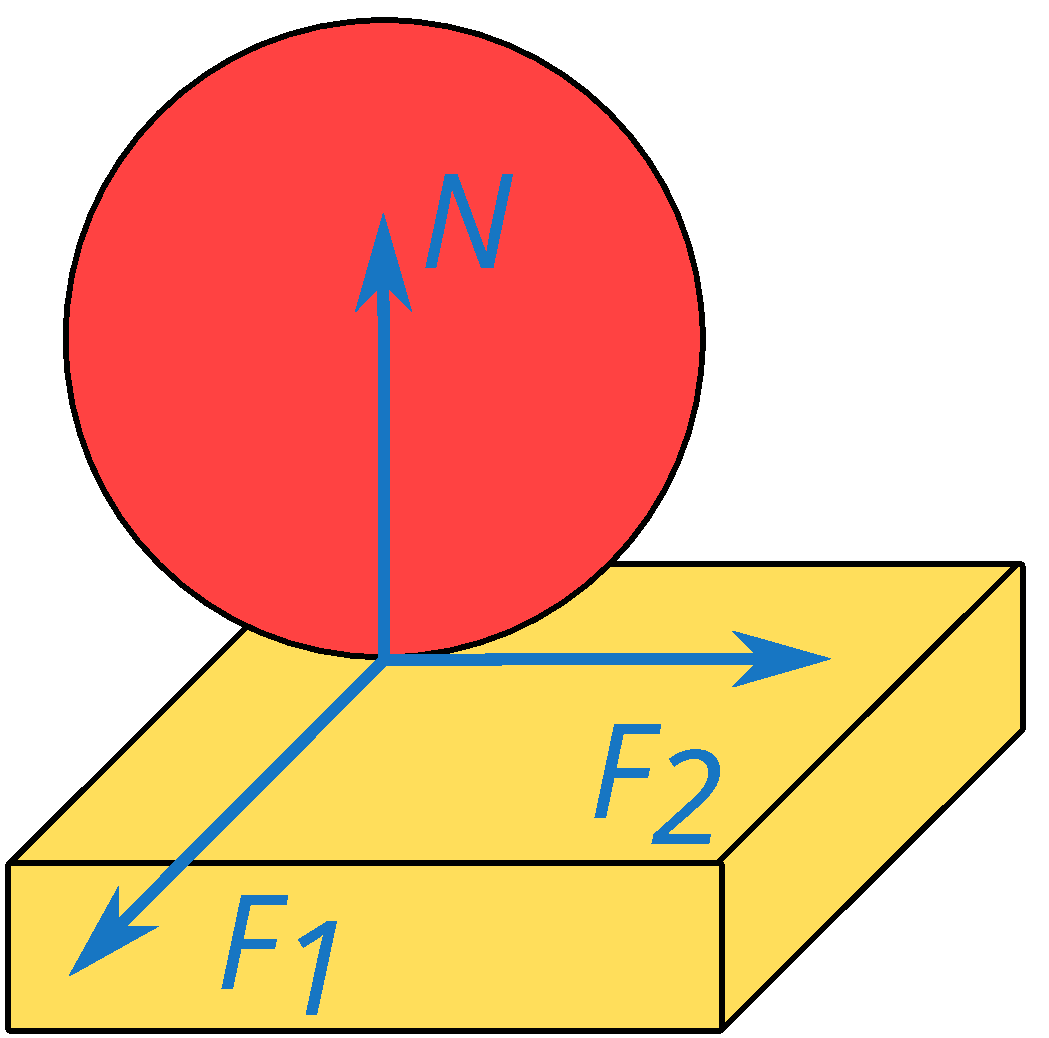
\includegraphics[width=0.5\textwidth]{graphics/friction.pdf}
		\caption{Wektory punktu kolizji.}
		\end{figure} 

		Po wykryciu punktu kolizji i wyznaczeniu wektora normalnych $N$ do dotykających się obiektów, system powinien zadziałać odpowiednimi siłami, 
		aby zatrzymać, lub odbić obiekty od siebie.
		Dodatkowo, ponieważ prędkości obiektów nie muszą być równoległe do wektora kolizji, należy zasymulować siłę tarcia z odpowiednią dla współczynnika tarcia wartością.
		Można to uzyskać, nadając obiektom w punkcie kolizji siłę prostopadłą do wektora normalnych, 
		ten wektor może być rozpisany przy pomocy dwóch wektorów jednostkowych $F_1$ i $F_2$. 
		Te wektory zawsze są prostopadłe do wektora normalnych, równoległe do płaszczyzny kolizji.

		W normalnej symulacji fizyki nigdy nie potrzeba osobno modyfikować współczynników tarcia i kierunku tych wektorów, 
		gdyż zazwyczaj powierzchnie symulowanych obiektów mają równe współczynniki tarcia w każdym kierunku.
		Jednakże modyfikując te wektory statycznie, lub dynamicznie, można uzyskać bardzo interesujące efekty.
		Instrukcja silnika symulacji podaje przykład, w którym aby zamodelować tarcie opon samochodu na zakręcie, prostopadle do kierunku jazdy, 
		należy dynamicznie zmieniać współczynnik tarcia dla wektora $F_1$, lub $F_2$ w kierunku promienia koła.
		Ten współczynnik tarcia, prostopadły do kierunku jazdy, może być liniowo zależny od prędkości.
		Spowoduje to, że im większa prędkość samochodu, tym boczna siła odśrodkowa bardziej wpłynie na tor jego jazdy, co ma odwzorowanie w rzeczywistości.
		Więcej informacji można znaleźć na stronie instrukcji maszyny symulacyjnej ODE \cite{ode_contact}.

		W opisywanym tutaj modelu, modyfikuje się wektor $F_1$, oraz współczynniki tarcia w obu kierunkach, aby przybliżyć zachowanie się rolki.
		Ponieważ wektory $F_1$ i $F_2$ są określone w lokalnym dla koła układzie współrzędnych, 
		w każdej iteracji maszyny symulacji należy obrócić je względem aktualnej pozycji bazy i odwrotności obrotu koła.
		Idealna rolka obraca się całkowicie bez tarcia, a ruch wzdłuż jej osi jest niemożliwy.
		Można więc ustawić zerowy współczynnik tarcia w kierunku prostopadłym do osi, oraz nieskończenie duży dla wektora równoległego do osi.

		\begin{figure}[H]
		\centering
		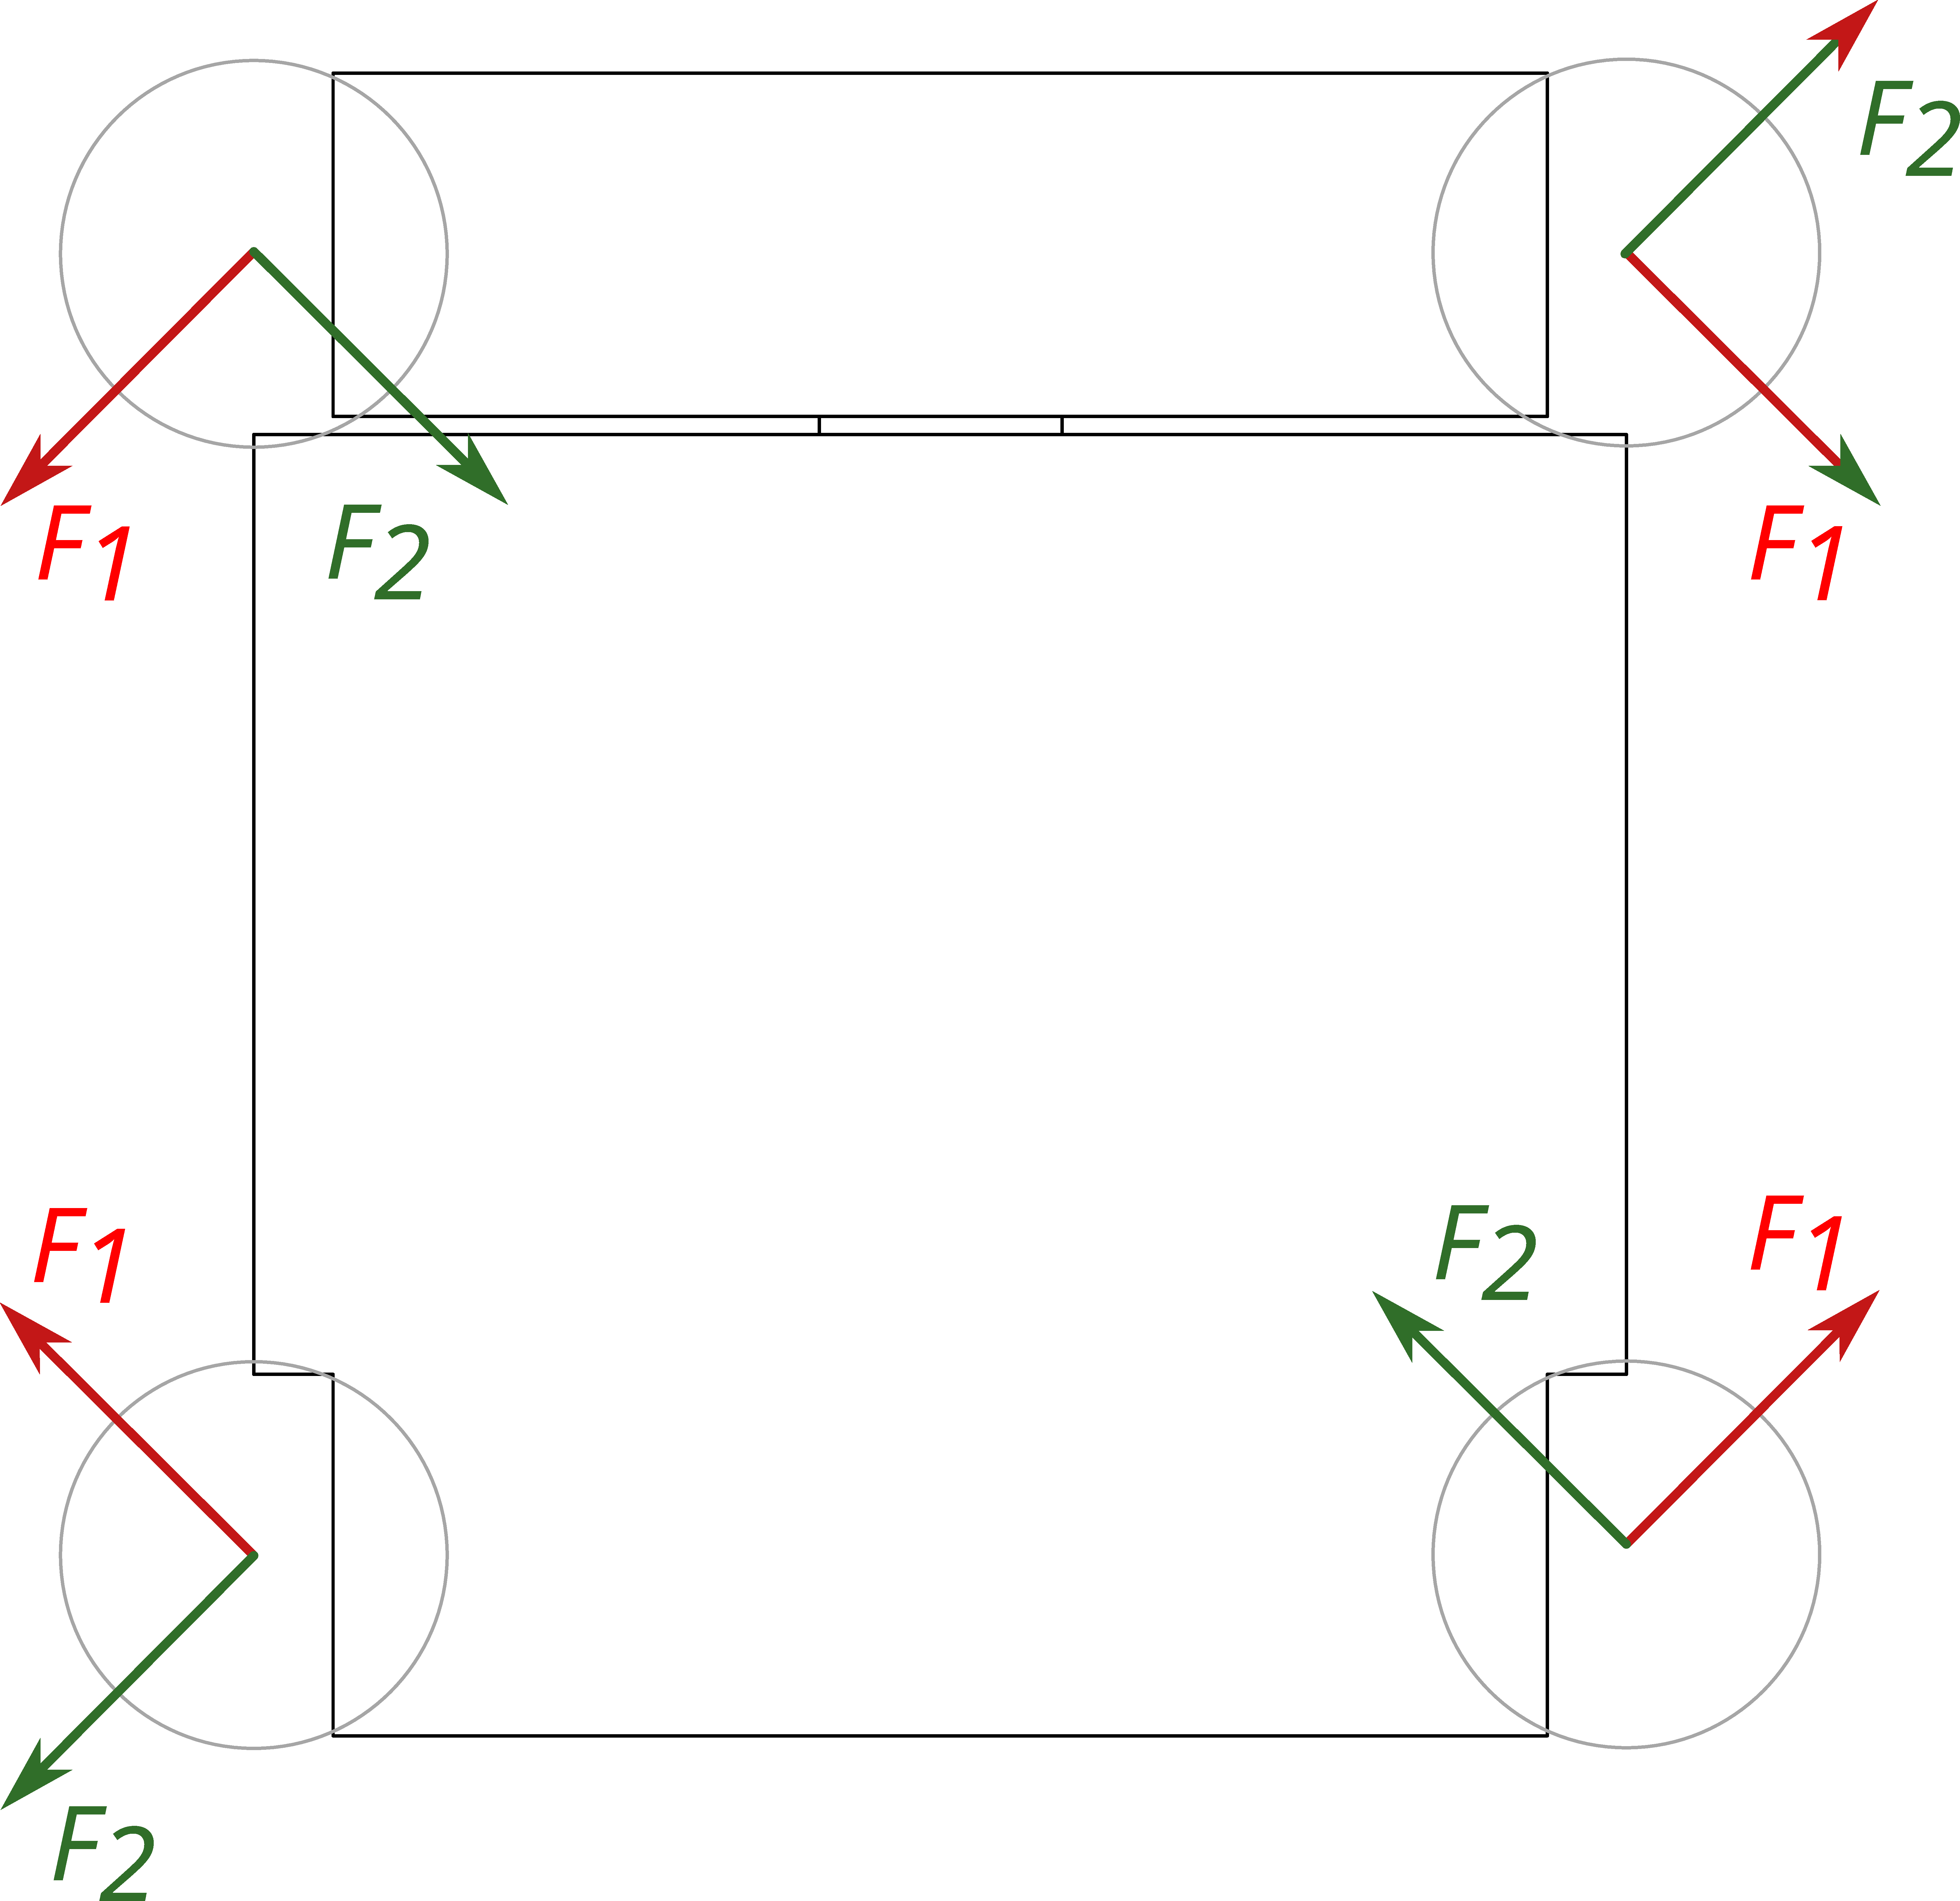
\includegraphics[width=0.8\textwidth]{graphics/base_vects.pdf}
		\caption{Kierunki wektorów dla których należy nadać współczynniki tarcia przy symulacji platformy, widok z góry. Tarcie w kierunku $F_1$ powinno być nieskończone, a w $F_2$ zerowe.}
		\end{figure} 

		Niestety, w rzeczywistości rolki wykonane są ze śliskiego plastiku, który zezwala na poślizg kół wzdłuż ich osi.
		Osie kolek również nie obracają się płynnie, trzeba użyć dużej siły, aby obrócić dowolną z nich, pod naciskiem platformy tarcie jest jeszcze większe.
		Każda rolka obraca się z innym tarciem wprowadzając kolejne zakłócenia.
		Podłoże po którym porusza się robot także nie jest tu bez znaczenia.
		Należy zatem wystawić interfejs do łatwej zmiany współczynników tarcia, aby później dobierać odpowiednie wartości na podstawie zachowania rzeczywistego robota.

		Podobnie, jak w poprzednich przypadkach, modeluje się tylko najniższą, dotykającą podłoża rolkę.
		Jak wcześniej wspomniano, ma ona bardzo skomplikowany kształt, lecz można przybliżyć całe koło kulą.
		Zatem w miejscu każdego koła zamontowana jest kula z dynamicznie modyfikowanym tarciem i siatką w kształcie koła do wizualizacji, 
		oraz przegub z motorem łączący odpowiednią część bazy z kołem.
		To najprostsza budowa modelu (a zatem najszybsza) z poprzednich.
		
		\begin{figure}[H]
		\dirtree{%
		.1 kadłub\DTcomment{Podstawa bazy}.
		.2 przegub z silnikiem\DTcomment{Nadaje moment obrotowy na żądanie}.
		.3 kula\DTcomment{Modyfikowane wektory tarcia}.
		.4 siatka\DTcomment{Odpowiada za wygląd obiektu koła}.
		}
		\caption{Zagnieżdżenie obiektów koła w strukturze drzewiastej z modyfikowanymi wektorami tarcia. W implementacji Gazebo przegub i kula są zagnieżdżone równolegle.}
		\label{fig:omnivelma_wheel}
		\end{figure}

		Takie rozwiązanie wiąże się z pewnym ryzykiem.
		Wymaga, aby symulator używał maszyny ODE, co zmniejsza przenośność modelu. ODE jest domyślnym symulatorem w Gazebo.
		Maszyna Bullet również liczy kolizje w ten sposób i ma modyfikowalne wektory, 
		lecz nie daje podobnych wyników. Być może jest to spowodowane brakiem odpowiedniej konfiguracji, lub innym wewnętrznym traktowaniem modelu.

	\subsection{Komunikacja}
		Ze względu na wiele ustawień elementów bazy, należy stworzyć bogaty interfejs.
		W każdym cyklu symulacji, program sterujący modelem platformy nadaje wiadomości:
		\begin{itemize}
		\item \texttt{geometry\_msgs/PoseStamped} z aktualną pozycją i rotacją platformy, oraz nagłówek z czasem i identyfikatorem.
		\item \texttt{geometry\_msgs/TwistStamped} z aktualną prędkością platformy i nagłówkiem.
		\item \texttt{omnivelma\_msgs/EncodersStamped} z odczytaną ze stanu obiektów kół aktualną rotacją i pozycją, z nagłówkiem. 
		To jest symulator enkoderów wbudowanych w silniki platformy.
		\end{itemize}
		
		Przyjmowane są także dane:
		\begin{itemize}
		\item \texttt{omnivelma\_msgs/Vels} z zadanymi prędkościami kół.
		\item Wywołanie ustawiające współczynniki tarcia wzdłuż wektorów $F_1$ i $F_2$.
		\item Wywołanie ustawiające masy i momenty obrotowe niektórych elementów składowych konstrukcji.
		\end{itemize}

	\subsection{Rozszerzenie modelu}
		\label{sec:model_nan}
		Ponieważ komputerowa reprezentacja liczby zmiennoprzecinkowej pozwala na zapisanie nie tylko liczbowych wartości, można rozszerzyć model o dodatkową funkcjonalność,
		wywoływaną wysłaniem do modelu cichej nie-liczby (\emph{NaN}) w wiadomości, w polu prędkości odpowiedniego koła. 
		Cicha nie-liczba powstaje w procesorze, w module operacji zmiennoprzecinkowych, przy przeprowadzaniu nieprawidłowych, 
		acz niekrytycznych obliczeń, na przykład dzielenie przez zero, lub dzielenie nieskończoności przez minus-nieskończoność 
		(także zapisywane jako forma liczby zmiennoprzecinkowej).
		Takie operacje nie powodują błędu programu, jedynie wynik w postaci nie-liczby propaguje przez wszystkie pozostałe operacje.

		Nadanie prędkości modelom w przestrzeni wirtualnej polega na wywołaniu odpowiedniej funkcji maszyny symulującej fizykę.
		Można zadać pytanie, jak zachowa się model, jeśli dla niektórych kół nie zmieniać prędkości po każdym odebraniu pakietu?

		Wobec tego, jeśli w pakiecie z nowymi prędkościami kół znajdzie się cicha nie-liczba, program sterujący nie nada nowej prędkości temu kołu.
		Jest to podobne do nadania tej samej prędkości, jaką posiada aktualnie obiekt koła (jaką zwróciłby enkoder).

		Zwraca to uwagę również na potrzebę, aby program do komunikacji z rzeczywistym robotem nie skończył się błędem po odebraniu jednej z takich nieokreślonych wiadomości.
		Ponieważ przekształca liczby zmiennoprzecinkowe, zawarte w ROSoswych pakietach, na dane zrozumiałe przez sterownik silnika, które zazwyczaj są liczbami
		stałoprzecinkowymi, program może zachować się nieprzewidywalnie.
